% TODO klar benennen, dass wir uns jetzt ein Fallbeispiel Anschauen

\begin{frame}{Die Vier Domänen der Sicherheit sind…}
  % GOAL Orientierung, wo wie gerade hinschauen für das Fallbeispiel
  \Large
  \begin{columns}[c]
    \begin{column}{.5\linewidth}
      \textbf{Luftfahrt}
    \end{column}
    \begin{column}{.5\linewidth}
      Automobile
    \end{column}
  \end{columns}
  \vfill
  \begin{columns}[c]
    \begin{column}{.5\linewidth}
      Medizintechnik
    \end{column}
    \begin{column}{.5\linewidth}
      Automatisierung
    \end{column}
  \end{columns}
\end{frame}

\interlude[1]{Kryptografie in der Avionik}

\begin{frame}[c]{Sichere Kryptografie in der Avionik}
  % TODO: Screenshot von Economy Class cryptography Paper, und von LDACS paper
  % TODO: Both papers in two-column?
  % GOAL Aufzeigen, das (gute) Cryptography in Avionik fehlt
  \vspace{4em}
  \footnotesize
  (Gähnende Leere)
\end{frame}

\begin{frame}[c]{Zum erschrecken aller…}
  % GOAL Aufzeigen, dass auch fortschrittliche Planung durch Mangelnde Kryptoagilität zum scheitern verurteilt ist (LDACS Paper)
  \begin{columns}[fullwidth,c]
    \begin{column}{.5\linewidth}
%      \begin{itemize}

        \footnotesize
        …wird in der Luftfahrt heutzutage keine sichere Kryptografie eingesetzt. 
%      \end{itemize}
    \end{column}%
    \begin{column}{.5\linewidth}
      % GOAL Digital Drahtlos Kommunikation seit 45 jahren
      % GOAL Erste ernste zunehmende Kryptographie in 2007 eingeführt, aber quasi keine Verbreitung
      % GOAL 2021 dann der erste Vorschlag, für einen hybridig post-quaten sicheren Datalink...
      % GOAL ... aber noch vor dem Rollout und nach nur einem Jahr ist die chiffre gebrochen :(
      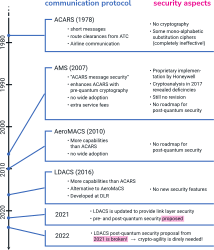
\includegraphics[width=.92\linewidth]{graphics/history of cryptography in avionics}
    \end{column}
  \end{columns}
\end{frame}


\begin{frame}[c]{Kryptographie in der Avionik: Ansatz}
  % GOAL HPKE ist ein standard  mit festen interface, dennoch sind die internen Primitive modular
  % TODO check graphics from slides from HACMAS
  % TODO größerere Graphic, in die mitte
  \begin{columns}[fullwidth,c]
    \begin{column}{.65\linewidth}
      \begin{itemize}
        \item HPKE-Standard als Basis

        \item Schnittstelle aus HPKE
        \begin{itemize}
          \item Seal: Nachricht verschlüsseln (und signieren)
          \item Open: Nachricht entschlüsseln (und prüfen)
        \end{itemize}

        \item Interne Umsetzung Modular basiert auf Modulen\\ % TODO fußnote an alles dranpacken
         (KEM, KDF \& AEAD\footnote{Avioniker und auch Kryptographen lieben Akronyme}) % TODO marei Fußnote zieht blauen balken hoch

        % \item Modularität der Primitive
        % \begin{itemize}
        %   \item KEM: Key Encapsulation Funktion\\Eigener Privater Schlüssel, Öffentlicher Schlüssel Addressat $\rightarrow$ Sym. Schlüssel
        %   \item KDF: Key Derivation Function\\Schlüsselmaterial, Entropie $\rightarrow$ Schlüssel
        %   \item AEAD: Authenticated Encryption with Associated Data\\
        %     Symetrische Chiffre mit Authentisierung\\
        %     Klartext, Sym. Schlüssel $\rightarrow$ Cyphertext\\
        %     Cyphertext, Sym. Schlüssel $\rightarrow$ Klartext. Authentisiert?
        % \end{itemize}

        % TODO placement and size of graphics
      \end{itemize}
    \end{column}%
    \begin{column}{.35\linewidth}
      
        \includegraphics[width=0.8\linewidth]{graphics/hpke}
        % TODO explain every detail of this Graphic
    \end{column}
  \end{columns}
\end{frame}


\begin{frame}[c]{Flexible Einsatzszenarien, gleiche Schnittstelle}
  % GOAL Auswahl der Primitive erlaubt tradeoffs, Schnittstelle bleibt gleich
  \begin{columns}[fullwidth,c]
    \begin{column}{.35\linewidth}
      \begin{itemize}
        \item Pre oder Post-Quantum?
        \item Mehr oder weniger Speicherbedarf?
        \item Schenelle or langsame Berechnung?
        \item Post-quantum Authentisierung? 
      \end{itemize}
    \end{column}%
    \begin{column}{.65\linewidth}
      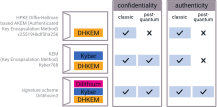
\includegraphics[width=\linewidth]{graphics/hpke variants}
    \end{column}
  \end{columns}
\end{frame}


\begin{frame}[c]{Partitionen zur Integration in die Avionik}
  % \begin{columns}[fullwidth,c]
  %   \begin{column}{.4\linewidth}
  %     \begin{itemize}
  %       \item Bündelung der Kyrypto-Implementierung
  %       \item Modul der Avionik: Partition\footnote{Partitionen sind voneinander isoliert, und dürfen daher in der Zulassung separat betrachtet werden}
  %       \item Einfacher Austausch der Krypto-Partition
  %     \end{itemize}
  %     \vspace{8.5em} % TODO This is a hack, maybe marei can fix it?
  %   \end{column}%
  %   \begin{column}{.6\linewidth}
      \centering 
      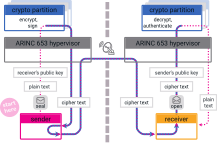
\includegraphics[width=0.8\linewidth]{graphics/crypto partition}
  %   \end{column}
  % \end{columns}
\end{frame}

% GOAL Aufzeigen, dass und wie Modularität der Schlüssel für Kryptoagilität in der Safety ist
% GOAL Aufzeigen, dass Integration einfach möglich, und zulassungsfreundlich gemacht werden kann


% TODO eine folie über Benchmarks?


% \begin{frame}[c]{Ansätze für Verbesserung in beiden Bereichen}
%   % GOAL ist mir unklar
%   % TODO wucke refine 

%   Verifikationstechniken
%   \vspace{0.5em}

%   {\footnotesize Zertifizierung <-> Sicherheitsbeweise}
%   \vspace{1.5em}
%   % Formaler Beweis kann Teil der Evidence für Zertifizierung sein
%   % Annahmen und Anforderungen müssen in den Zertifizierungsdokumenten festgehalten werden
%   % Evidence = Belege, warum Annahmen wahr sind oder Anforderungen erfüllt sind
%   % Unabhängigkeit zwischen Implementierer und Verifizierer
%   % 
%   % - Wanja
%   %
%   % Agreed; geht mir eher darum die generelle Vorgehensweise zu beschreiben als formell korrekt jede Möglichkeit durchzugehen.
%   % Ist beweisführung in der Avionik denn üblich?
%   % 
%   % – Karolin

%   Kompartmentalisierung
%   \vspace{0.5em}

%   {\footnotesize Partitionierung <-> Brokerarchitekturen}
%   \vspace{1.5em}
%   % Aufteilung erleichtert sukzessive Absicherung einzelner Komponent
%   % Gleichzeitig: Faultcontainment
%   % Modularisierung macht updates einfacher, da klare interfaces zwischen Modulen

%   % Diagram Idee: Konfidenzarchitektur
%   %
%   % 1. Identifiziere mögliche Fehlerursachen
%   % 2. Ist ein Fehler relevant?
%   %   - Falls Nein, warum nicht? Evidence!
%   % 3. Welche Effekte hat der Fehler?
%   % 4. Wie kann der Fehler verhindert/eingedämmt/mitigiert werden?
%   % 5. Wie kann der Fehler erkannt werden?
%   % 6. Validiere Annahmen von 3. - 5.
%   % 7. Review durch unabhängigen Assesor
%   %
%   % -- wucke13
%   %
%   % Passt das denn in das Gegenüberstellungsscheme? Also wie bringen wir den Vergleich Avionik vs Crypto rein.
%   %
%   % -- karolin

%   => Kryptoagilität
% \end{frame}
